\begin{document}

\chapter{Implementation}

In this chapter I will discuss how this project is structured, going through the high-level details of the actual implementation that respects all the requirements defined in Section \ref{Requirement Analysis}. It will review how the initial data is processed and how the extracted features of interest are used with a view to creating further synthetic and real datasets. Furthermore, the chapter examines how the Patchy-San algorithm operates on graph inputs in order to create suitable NNs training data and thus, how the NNs architectures are designed and optimised for the given classification task. Finally, the way in which files are renamed and reorganised into a virtual filesystem are analysed. \\


\section{Data Analysis and Processing}

\subsection{Data Properties}

\begin{figure}[H]
  \centering
  \centerline{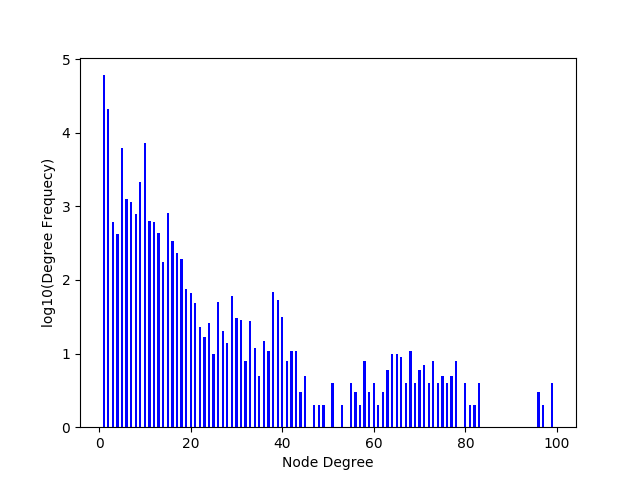
\includegraphics[scale = 0.86]{Images/nodedegdist.png}}
  \caption{Node degree distribution in Neo4J database.}
  \label{nodedegdist}
\end{figure}

\subsection{Neo4J Interaction and Feature Extraction}

\subsection{Feature Engineering}

\subsection{Synthetic Data Generation} \label{synthetic data generation}


\section{Overall Structure of the Project}

\begin{figure}[H]
  \centering
  \centerline{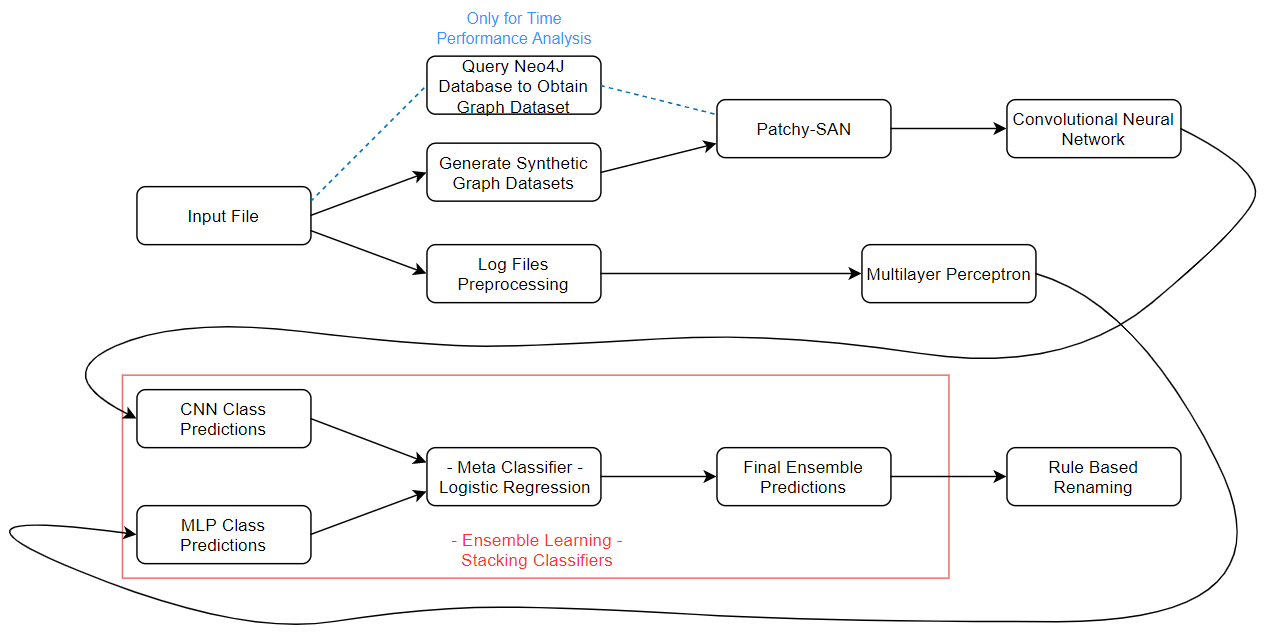
\includegraphics[scale = 0.6]{Images/pipeline.png}}
  \caption{Overview of the implemented ML pipeline.}
  \label{pipeline}
\end{figure}

\begin{figure}[H]
  \centering
  \centerline{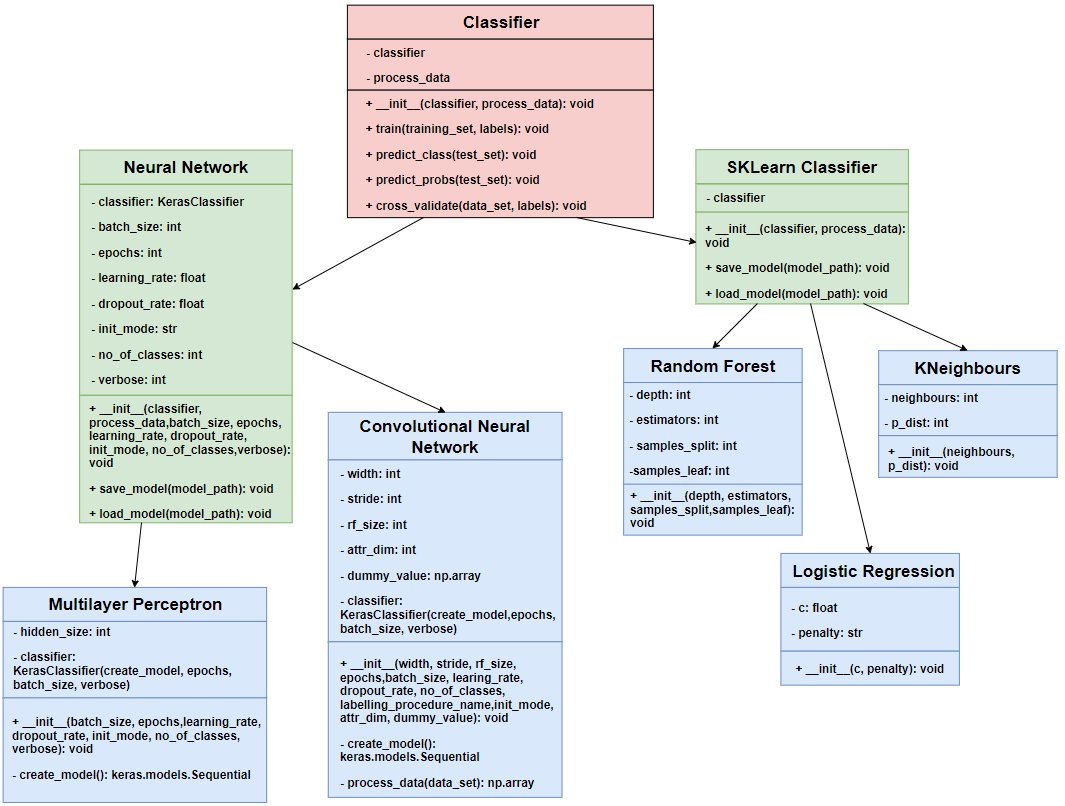
\includegraphics[scale = 0.7]{Images/uml.png}}
  \caption{UML diagram illustrating the inheritance of implemented classifiers.}
  \label{OOP}
\end{figure}

\subsection{Overview of the Renaming Pipeline}

\subsection{Nested Cross-Validation}

The fundamental success criteria of the project were to develop, tune and evaluate a ML pipeline capable of classifying files in term of both content and provenance graph. In order to deal with the second and third mentioned goals, I have implemented a Nested Cross-Validation (CV) procedure. A detailed description of how it is performed follows and an expressive visualisation of it can be observed in Figure \ref{NestedCV}. \bigskip

\begin{itemize}[label={}]
  \item 1. divide the dataset into K stratified cross-validation folds at random
  \item 2. for each fold $k$ = 1,2,...,K (outer loop for evaluation of the model with selected hyperparameter):
        \begin{itemize}[label={}]
          \item 2.1. let fold $k$ be the outer test set
          \item 2.2. let all data except for fold $k$ be the outer training set
          \item 2.3. randomly split training set into L stratified fold
          \item 2.4. for each fold $l$ = 1,2,...,L (inner loop for hyperparameter tuning):
                \begin{itemize}[label={}]
                  \item 2.4.1. let fold $l$ be the inner validation set
                  \item 2.4.2. let all data except fold $k$ and fold $l$ be the inner training set
                  \item 2.4.3. train with each hyperparameter on inner training set and evaluate on fold $l$, keeping track of performance metrics
                \end{itemize}
          \item 2.5. for each hyperparameter setting, calculate average metrics score over the L folds and choose the best one
          \item 2.6. train a model with the best hyperparameter on fold $k$, evaluate its performance and save its score
        \end{itemize}
  \item 3. calculate the mean score over all K folds and report as the generalisation error
\end{itemize} \bigskip

An outer CV procedure is performed to provide a performance estimate used to select the optimal model. In each fold of the outer CV, the hyperparameters of the model are tuned independently to maximise an inner CV estimate of generalisation performance. The outer CV is then essentially estimating the performance of a method for fitting a model, CV based hyperparameter tuning. This eliminates the bias introduced by a flat CV procedure as the test data in each iteration of the outer CV has not been used to optimise the performance of the model in any way, and may therefore provide a more reliable criterion for choosing the best model. Another advantage consists of tuning and evaluating on the entire dataset, instead of completely discarding the validation set. The computational expense of nested CV, however, is substantially higher. \\



\begin{figure}[H]
  \centering
  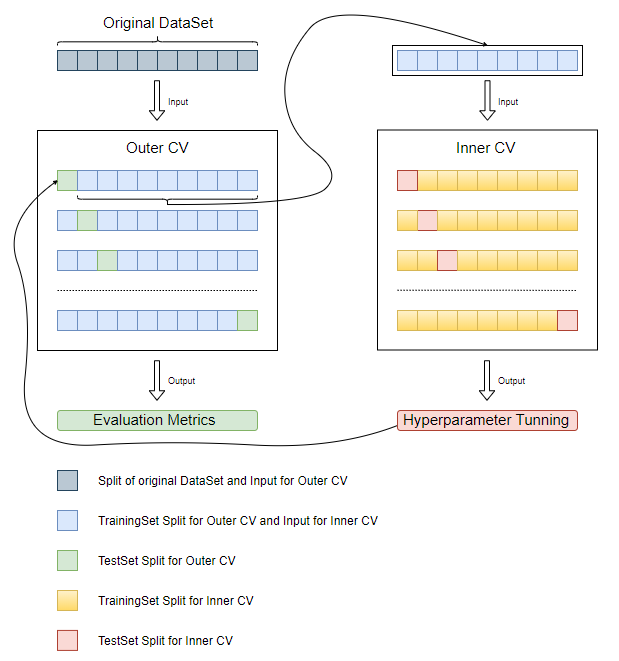
\includegraphics[scale=0.95]{Images/nested_cv.png}
  \caption{Structure of a Nested Cross-Validation used for both model evaluation and hyperparameter tuning.}
  \label{NestedCV}
\end{figure}


\section{Patchy-San}

Patchy-San aims to bring CNNs to bear on a large-class of graph based learning problems. This novel algorithm consists of a general approach of extracting locally connected regions from graphs and model them in such a way so that they become a suitable input for a CNN. In this context, suitable refers to both structurally adequate and having the capability of preserving graph's expressivity, in the sense that local pattern information is not lost when linearising the set of features. \\

My re-implementation brings a few adjustments and extensions (mentioned in the upcoming sections) to the original algorithm so that it suits better the shape and properties of the dataset provided. \\

\subsection{Node Sequence Selection}

The first step in the algorithm consists of establishing a node ordering for the input graph based on a chosen graph labelling function. In general, any reasonable graph labelling function would work for this sorting procedure. For instance, an artificial, independent of dataset knowledge approach, can use the betweenness centrality value of each node. However, given the insights into the provenance dataset, I chose to use the timestamp of the influence relations for labelling purposes, as this would imply a more natural ordering and actually improve the overall results. \\

Given this ordering, a subset of nodes is designated as the roots (Node Sequence) from where the actual receptive fields will be constructed. Specifically, each two consecutive picked roots from the sorted list of nodes are within a constant distance from each other. This distance ($s$) is called a stride. The aim is to construct the same $w$ number of receptive fields for each input graph as they will be provided as training/testing data for the convolutional neural network. Therefore, in case the number of nodes is not sufficient for building $w$ receptive fields, the algorithm creates all-zero receptive fields for padding purposes. \\

\begin{figure}[H]
  \centering
  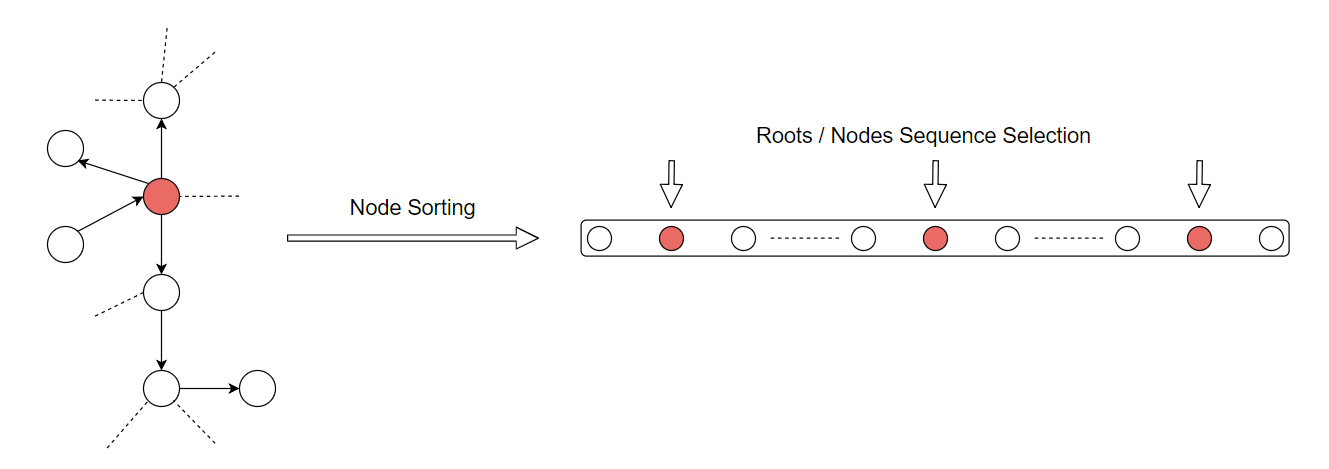
\includegraphics[scale=0.5]{Images/nodeseqsel.png}
  \caption{Input graph node's sorted with respect to the labelling function. $w$ root nodes selected within stride $s$.}
  \label{nodeseqsel}
\end{figure}

\subsection{Neighbourhood Assembly}

The next stage involves assembling a local neighbourhood for each root previously determined. This is accomplished by using a standard breath-first search algorithm. Thus, I explore vertices with an increasing distance from the root, adding them to a set N. If the number of collected nodes is smaller than a pre-established number $k$, I continue exploring the immediate neighbours of the latest nodes added to the set until either $k$ nodes are found, or there are no more neighbours. In the latter case, for padding purposes, dummy nodes, having dummy attributes are added. This helps not throwing away information that might convey in-graph patters. However, it introduces the risk of misidentifying the padding nodes as a pattern themselves. \\

One final remark for the neighbourhood assembly procedure is that the order in which the immediate neighbours of a node are explored is with respect to, once again, the timestamp of each influence edge. Specifically, newer system activities will be considered with priority, also ensuring that the procedure is consistent and always gives the same output for the same graph. \\

\begin{figure}[H]
  \centering
  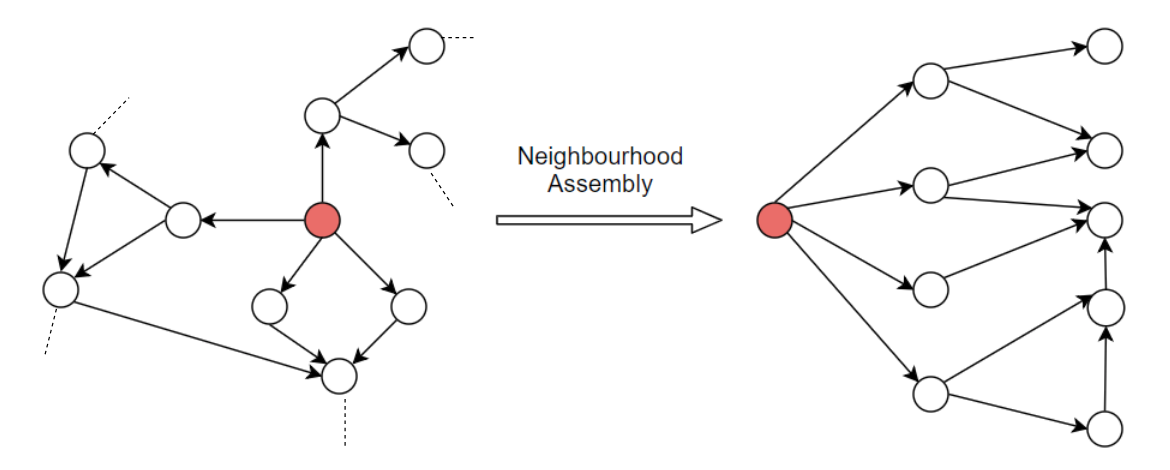
\includegraphics[scale=0.375]{Images/neighassemb2.png}
  \caption{Illustration of a Breath-First Search used for computing a neighbourhood.}
  \label{neighassemb}
\end{figure}


\subsection{Receptive Field Normalisation}

The receptive field of a node is built by normalising the neighbourhood assembled in the previous step. The normalisation imposes an order on the nodes of the neighbourhood graph so as to map from the unordered graph space to a vector space with a linear order. This time, the graph labelling procedure is way more difficult to compute, as appropriately choosing it is at the core of the representation that Patchy-San proposes. Hence the performance of the classification pipeline will highly depend on the labelling procedure. \\

The basic idea is that the graph labelling procedure should assign nodes of two different graphs in similar positions if and only if they have similar structural roles in the graphs. The labelling of the vertices is therefore constrained by the graph distance to the root node $v$. For any two vertices $u$, $w$, if $u$ is closer to $v$ than $w$, then $v$ is
always ranked higher than $w$. This definition, illustrated in Figure \ref{normalisation}, ensures that $v$ has always rank 1, and that the closer a vertex is to $v$ in the graph, the higher it is ranked in the vector space representation. Consequently, in my project, this implies that groups of nodes denoting: processes interacting directly with the file to be classified, parent processes of the ones just mentioned, past processes interacting with the file at different moments in time; will be close together in the linear representation and also in same order for different graphs.\\

\begin{figure}[H]
  \centering
  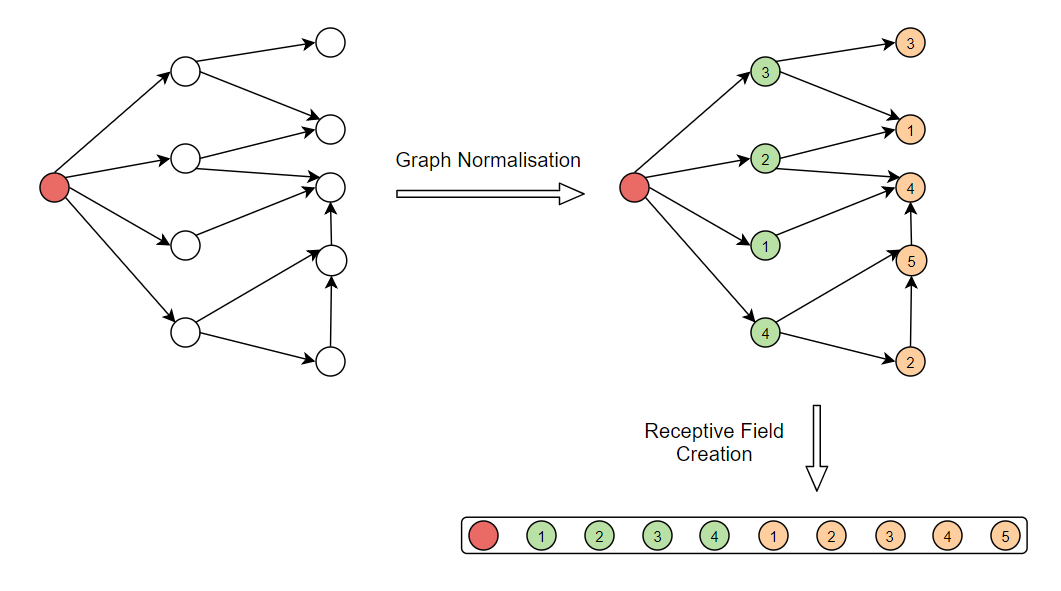
\includegraphics[scale=0.55]{Images/normalisation.png}
  \caption{Receptive Field Normalisation from previously selected neighbourhood. Nodes having the same colour have the same rank with respect to root in the liniarisation, while numbers illustrate tie-breakers.}
  \label{normalisation}
\end{figure}

One important detail that was taken into account is that, in general, the described labelling procedure does not consist of an injective function, thus a method to break ties between same-labelled nodes is necessary.

\section{Convolutional Neural Network}

For each input graph $G$, given the construction of the receptive fields, and the number of attributes of each vertex $a_v$, I compute an initial 3D tensor of sizes ($w$, $k$, $a_v$), which is afterwards reshaped to a 2D tensor ($wk$, $a_v$) and fed as input for the CNN (where, obviously, $a_v$ will be the number of input channels). \\

\subsection{Parameter initialisation}

The initial values of the parameters of a NN drastically influence the quality of the solution returned by the mini batch gradient descent optimisation algorithm, as they may direct the process towards different local minima. NN's weights receive an update proportional to the partial derivative of the error function with respect to the current weight in each iteration of training. Therefore, if the initial weights are too small, they will shrink exponentially as they go deeper and deeper into the network, until they vanish. This situation severely reduces NN's capacity of representing non-linearities. On the other hand, if the initial weights are too large, they will grow exponentially larger as they go deeper and deeper into the network, until they might overflow, crashing the model. Even if the parameters don't overflow, the layers can still become insanely large, resulting in the algorithm diverging. Bearing these two aspects in mind, the aim is to distribute the initial parameters in such a manner that they can successfully (i.e. not vanishing nor exploding) travel forwards and backwards withing the network. \\

The initialisation strategy used for the CNN is He initialisation and consists of ...\\

The initialisation strategy used for the MLP is called Xavier initialisation. It takes into account the problems shown above and bases the standard deviation or the variance of the weight initialisation on the number of variables involved. It thereby adjusts itself based on the number of weight values. It works on the idea that if the variance is kept constant from layer to layer in both the feed forward direction and back-propagation direction, the network will learn optimally. Specifically, this method initialises weights by drawing them from a small Gaussian distribution with: \\

\begin{equation}
  \centering
  \mu = 0 \ \text{and} \ \sigma^2 = \frac{2}{n_{in}}
\end{equation}

where $n_{in}$ is the number of neurons which serve as input for the layer to which the weight belongs. \\

\begin{figure}[H]
  \centering
  \centerline{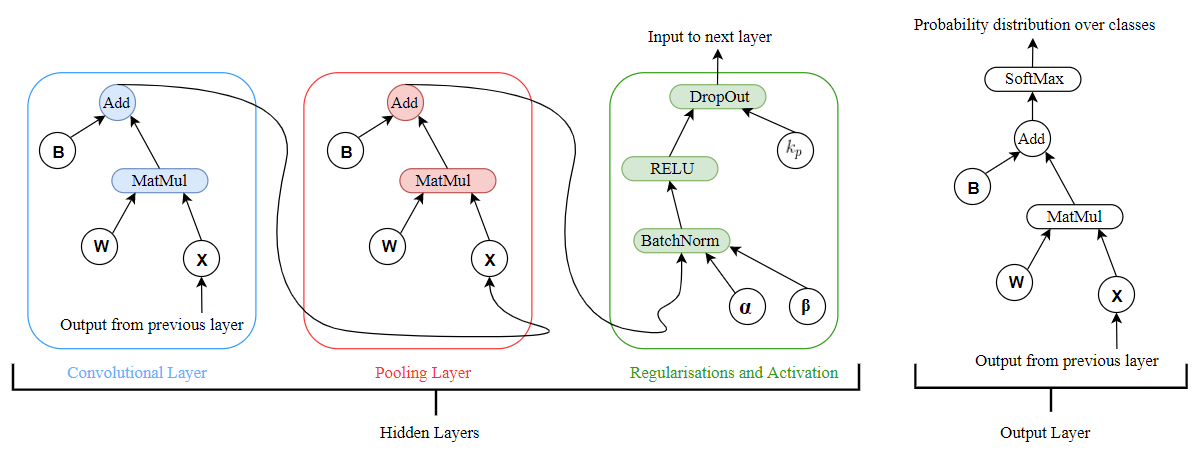
\includegraphics[scale=0.6]{Images/cnn_layers.png}}
  \caption{Diagram illustrating the configuration of hidden and output layers of the CNN.}
  \label{cnn_layers}
\end{figure}

     \begin{figure}[H]
  \centering
  \centerline{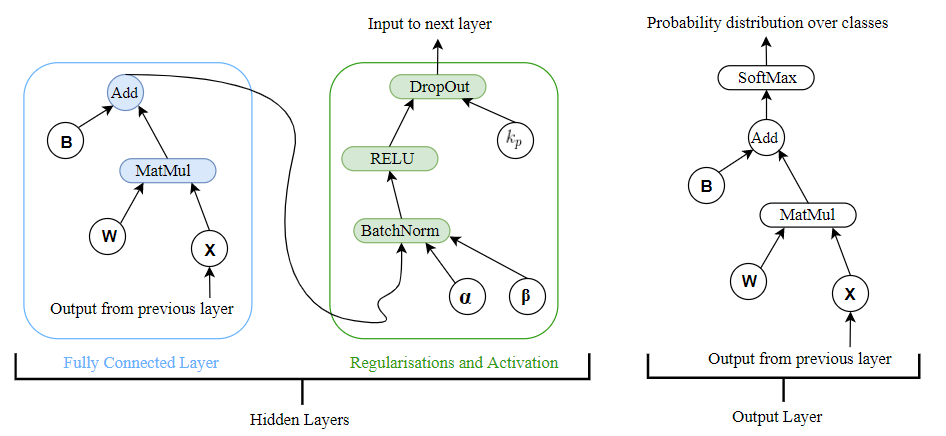
\includegraphics[scale=0.6]{Images/mlp_layers.png}}
  \caption{Diagram illustrating the configuration of hidden and output layers of the MLP.}
  \label{mlp_layers}
    \end{figure}

\section{Regularisation Techniques}

Deep NNs can be trained to develop complex relationships between their input data and their outcome. Depending on the amount of training data the network may develop a behaviour that brings good results for the training data, but fails as soon as unknown test data is fed into the network. To prevent overfitting in neural networks, there exist a variety of methods. A few of them were implemented and are discussed in this section.

\subsection{Dropout}

Dropout is a regularisation technique behaving in the following manner: on each training iteration, a randomly chosen subset of neurons in the NN are shut down, in the sense that the NN will perform forward propagation and back-propagation as if those nodes (alongside with their inwards and outwards edges) are not preset at all. Since the units that are dropped out in each iteration are random, this forces the learning algorithm to spread out the weights and not focus on some specific features. This procedure can be visualised in Figure \ref{dropout}. In the simplest case, each unit is retained with a fixed probability $p$ independent of other units, which is introduced as a new hyperparameter in the NN. \\

One important aspect to note is that the weights of the network will be larger than normal because of dropout. Thus, if a unit is retained with probability $k_p$ during training, the outgoing weights of that unit are multiplied by $p$ at test
time. Another approach is to re-scale weights at training time instead, after each weight update at the end of the mini-batch. This is sometimes called inverse dropout and is the way both Keras and Pytorch deep learning libraries implement it. \\


\begin{figure}[H]
  \centering
  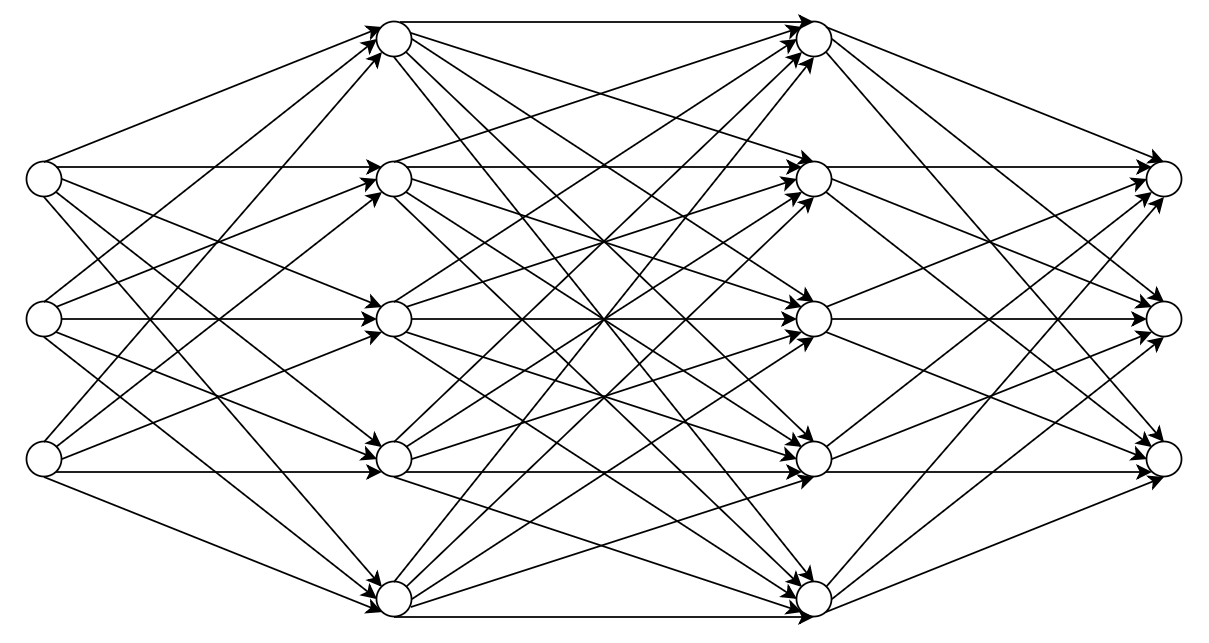
\includegraphics[scale=0.35]{Images/beforedrp.png}

  \bigskip

  \bigskip

  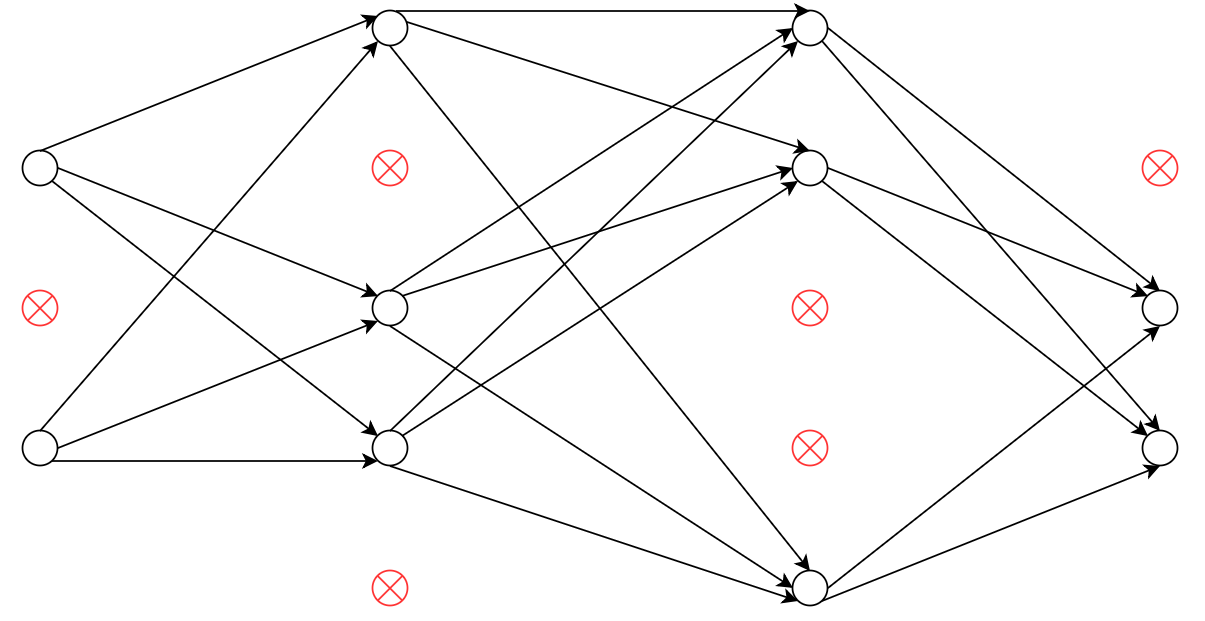
\includegraphics[scale=0.35]{Images/afterdrp.png}

  \bigskip

  \caption{Neural Network before (upper image) and after (lower image) dropout.}
  \label{dropout}
\end{figure}

\subsection{Batch Normalisation}


One of the key motivations for the development of Batch Normalisation was the reduction of so-called internal covariate shift (ICS). ICS is the phenomenon wherein the distribution of inputs to a layer in the NN changes due to an update of parameters in the previous layers. This change leads to a constant shift of the underlying training problem and is thus believe to have detrimental effect on the training process. \\

Therefore, Batch Normalisation is a mechanism that aims to stabilise the distribution (over a mini-batch) of inputs \{$x_1$, $x_2$, ... , $x_n$\} to a given NN during training. This is achieved by augmenting the NN with additional layers that set the first two moments: mean - $\mu = \frac{1}{n} \sum_{i=1}^n x_i$ and variance - $\sigma = \sqrt{\frac{1}{n} \sum_{i=1}^n (x_i - \mu) ^ 2}$, of the distribution of each activation to be zero and one respectively. Thus, it normalises the inputs in the following manner: \\

\begin{equation}
  \centering
  \hat{x}_k = \frac{x_k - \mu}{\sqrt{\sigma + \epsilon}}
\end{equation}

where $\epsilon > 0$ is a small constant added to avoid division by 0. \\

Then, the batch normalised inputs are also typically scaled and shifted based on trainable parameters $\gamma$ and $\beta$ to preserve model expressivity. \\

\begin{equation}
  \centering
  y_k = \gamma_k * \hat{x}_k + \beta_k
\end{equation}

\subsection{Weight Decay}
Weight decay is a standard trick to improve the generalisation performance of neural
networks by constraining the weights to be small in magnitude and penalizing large weights. Specifically, weight decay is defined as multiplying each weight in the gradient descent at each epoch by a factor $\lambda$ smaller than one and greater than zero. This technique is equivalent to introducing an L2 regularisation term to the loss function that one wants to optimise. Therefore, the updated loss functions will be of the following form: \\

\begin{equation}
  \centering
  \mathfrak{L}_{updated} = \mathfrak{L}_{model} + \frac{\lambda}{2} \norm{\textbf{w}}
\end{equation}

where $\norm{\textbf{w}} = \sqrt{\sum |w_i^2|}$ is the L2 norm of the weights vector.\\

Keras provides a weight regularisation API that allows one to add a penalty for weight size to the loss function. A weight regularizer can be added to each layer when the layer is defined in a Keras model. This is achieved by setting the $kernel\_regularizer$ argument on each layer.

\subsection{Early Stopping}
A problem with training neural networks is in the choice of the number of training epochs to use. Too many epochs can lead to overfitting of the training dataset as well as high training times, whereas too few may result in an underfit model. Early stopping is a method that allows one to specify an arbitrary large number of training epochs and stop training once the model performance stops improving on a hold out validation dataset. The error on the validation set is used as a proxy for the generalisation error in determining when overfitting has begun (i.e. the moment that after achieving a minimum, the error on the validation set starts increasing again).\\

Keras supports the early stopping of training via a callback called EarlyStopping. This callback requires setting the performance measure to monitor (hence defining what is considered to be an improvement), the trigger, and once triggered, it will stop the training process. In Keras, callbacks provide a way to execute code and interact with the training model process automatically. Callbacks can be provided to the \textit{fit()} function via the \textit{callbacks} argument. Often, the first sign of no further improvement may not be the best time to stop training. This is because the model may coast into a plateau of no improvement or even get slightly worse before improving considerably. We can account for this by adding a delay to the trigger in terms of the number of epochs on which we would like to see no improvement. This can be done by setting the \textit{patience} argument. \\


\section{Renaming the Files}

\section{Building a Virtual File System}


\section{Summary}


\end{document}